%%%%%%%%%%%%%%%%%%%%%%%%%%%%%%%%%%%%%%%%%
% Masters/Doctoral Thesis 
% LaTeX Template
% Version 2.5 (27/8/17)
%
% This template was downloaded from:
% http://www.LaTeXTemplates.com
%
% Version 2.x major modifications by:
% Vel (vel@latextemplates.com)
%
% This template is based on a template by:
% Steve Gunn (http://users.ecs.soton.ac.uk/srg/softwaretools/document/templates/)
% Sunil Patel (http://www.sunilpatel.co.uk/thesis-template/)
%
% Template license:
% CC BY-NC-SA 3.0 (http://creativecommons.org/licenses/by-nc-sa/3.0/)
%
%%%%%%%%%%%%%%%%%%%%%%%%%%%%%%%%%%%%%%%%%

%----------------------------------------------------------------------------------------
%	PACKAGES AND OTHER DOCUMENT CONFIGURATIONS
%----------------------------------------------------------------------------------------

\documentclass[
11pt, % The default document font size, options: 10pt, 11pt, 12pt
%oneside, % Two side (alternating margins) for binding by default, uncomment to switch to one side
english, % ngerman for German
singlespacing, % Single line spacing, alternatives: onehalfspacing or doublespacing
%draft, % Uncomment to enable draft mode (no pictures, no links, overfull hboxes indicated)
%nolistspacing, % If the document is onehalfspacing or doublespacing, uncomment this to set spacing in lists to single
%liststotoc, % Uncomment to add the list of figures/tables/etc to the table of contents
%toctotoc, % Uncomment to add the main table of contents to the table of contents
%parskip, % Uncomment to add space between paragraphs
%nohyperref, % Uncomment to not load the hyperref package
headsepline, % Uncomment to get a line under the header
%chapterinoneline, % Uncomment to place the chapter title next to the number on one line
%consistentlayout, % Uncomment to change the layout of the declaration, abstract and acknowledgements pages to match the default layout
openany
]{MastersDoctoralThesis} % The class file specifying the document structure

\usepackage[utf8]{inputenc} % Required for inputting international characters
\usepackage[T1]{fontenc} % Output font encoding for international characters

\usepackage{mathpazo} % Use the Palatino font by default

\usepackage[backend=bibtex,style=authoryear,natbib=true]{biblatex} % Use the bibtex backend with the authoryear citation style (which resembles APA)

\addbibresource{master-thesis.bib} % The filename of the bibliography

\usepackage[autostyle=true]{csquotes} % Required to generate language-dependent quotes in the bibliography

\newcommand*{\captionsource}[2]{%
  \caption[{#1}]{%
    #1%
    \\\hspace{\linewidth}%
    \textbf{Source:} #2%
  }%
}

%----------------------------------------------------------------------------------------
%	MARGIN SETTINGS
%----------------------------------------------------------------------------------------

\geometry{
	paper=a4paper, % Change to letterpaper for US letter
	inner=2.5cm, % Inner margin
	outer=3.8cm, % Outer margin
	bindingoffset=.5cm, % Binding offset
	top=1.5cm, % Top margin
	bottom=1.5cm, % Bottom margin
	%showframe, % Uncomment to show how the type block is set on the page
}

%----------------------------------------------------------------------------------------
%	THESIS INFORMATION
%----------------------------------------------------------------------------------------

\thesistitle{Central pattern generator model using Spiking neural networks} % Your thesis title, this is used in the title and abstract, print it elsewhere with \ttitle
\supervisor{Sergiy \textsc{Yakovenko}} % Your supervisor's name, this is used in the title page, print it elsewhere with \supname
\examiner{} % Your examiner's name, this is not currently used anywhere in the template, print it elsewhere with \examname
\degree{Master of Science} % Your degree name, this is used in the title page and abstract, print it elsewhere with \degreename
\author{Yuriy \textsc{Pryyma}} % Your name, this is used in the title page and abstract, print it elsewhere with \authorname
\addresses{} % Your address, this is not currently used anywhere in the template, print it elsewhere with \addressname

\subject{Data Science} % Your subject area, this is not currently used anywhere in the template, print it elsewhere with \subjectname
\keywords{CPG, Nengo, SNN} % Keywords for your thesis, this is not currently used anywhere in the template, print it elsewhere with \keywordnames
\university{\href{http://www.ucu.edu.ua}{Ukrainian Catholic University}} % Your university's name and URL, this is used in the title page and abstract, print it elsewhere with \univname
\department{\href{http://department.university.com}{Faculty of Applied Sciences}} % Your department's name and URL, this is used in the title page and abstract, print it elsewhere with \deptname
\group{\href{http://researchgroup.university.com}{Department of Computer Sciences}} % Your research group's name and URL, this is used in the title page, print it elsewhere with \groupname
\faculty{\href{http://faculty.university.com}{}} % Your faculty's name and URL, this is used in the title page and abstract, print it elsewhere with \facname

\AtBeginDocument{
\hypersetup{pdftitle=\ttitle} % Set the PDF's title to your title
\hypersetup{pdfauthor=\authorname} % Set the PDF's author to your name
\hypersetup{pdfkeywords=\keywordnames} % Set the PDF's keywords to your keywords
}

\begin{document}
\frontmatter % Use roman page numbering style (i, ii, iii, iv...) for the pre-content pages

\pagestyle{plain} % Default to the plain heading style until the thesis style is called for the body content

%----------------------------------------------------------------------------------------
%	TITLE PAGE
%----------------------------------------------------------------------------------------

\begin{titlepage}
\begin{center}

\vspace*{.06\textheight}
{\scshape\LARGE \univname\par}\vspace{1.5cm} % University name
\textsc{\Large Master Thesis}\\[0.5cm] % Thesis type

\HRule \\[0.4cm] % Horizontal line
{\huge \bfseries \ttitle\par}\vspace{0.4cm} % Thesis title
\HRule \\[1.5cm] % Horizontal line
 
\begin{minipage}[t]{0.4\textwidth}
\begin{flushleft} \large
\emph{Author:}\\
\href{http://www.johnsmith.com}{\authorname} % Author name - remove the \href bracket to remove the link
\end{flushleft}
\end{minipage}
\begin{minipage}[t]{0.4\textwidth}
\begin{flushright} \large
\emph{Supervisor:} \\
\href{http://www.jamessmith.com}{\supname} % Supervisor name - remove the \href bracket to remove the link  
\end{flushright}
\end{minipage}\\[3cm]
 
\vfill

\large \textit{A thesis submitted in fulfillment of the requirements\\ for the degree of \degreename}\\[0.3cm] % University requirement text
\textit{in the}\\[0.4cm]
\groupname\\\deptname\\[2cm] % Research group name and department name
 
\vfill

\includegraphics[height=4cm]{images/UCU-Apps.png} % University/department logo - uncomment to place it

\vfill
{\large Lviv 2020}\\[4cm] % Date
 
\vfill
\end{center}
\end{titlepage}

%----------------------------------------------------------------------------------------
%	DECLARATION PAGE
%----------------------------------------------------------------------------------------

\begin{declaration}
\addchaptertocentry{\authorshipname} % Add the declaration to the table of contents
\noindent I, \authorname, declare that this thesis titled, \enquote{\ttitle} and the work presented in it are my own. I confirm that:

\begin{itemize} 
\item This work was done wholly or mainly while in candidature for a research degree at this University.
\item Where any part of this thesis has previously been submitted for a degree or any other qualification at this University or any other institution, this has been clearly stated.
\item Where I have consulted the published work of others, this is always clearly attributed.
\item Where I have quoted from the work of others, the source is always given. With the exception of such quotations, this thesis is entirely my own work.
\item I have acknowledged all main sources of help.
\item Where the thesis is based on work done by myself jointly with others, I have made clear exactly what was done by others and what I have contributed myself.\\
\end{itemize}
 
\noindent Signed:\\
\rule[0.5em]{25em}{0.5pt} % This prints a line for the signature
 
\noindent Date:\\
\rule[0.5em]{25em}{0.5pt} % This prints a line to write the date
\end{declaration}

\cleardoublepage

%----------------------------------------------------------------------------------------
%	QUOTATION PAGE
%----------------------------------------------------------------------------------------

\vspace*{0.2\textheight}

\noindent\enquote{\itshape Thanks to my solid academic training, today I can write hundreds of words on virtually any topic without possessing a shred of information, which is how I got a good job in journalism.}\bigbreak

\hfill Dave Barry

%----------------------------------------------------------------------------------------
%	ABSTRACT PAGE
%----------------------------------------------------------------------------------------

\begin{abstract}
\addchaptertocentry{\abstractname} % Add the abstract to the table of contents
In this paper, we try to use a network of spiking neurons to build a Central Pattern Generator (CPG) model of a biological system. The classical approach for this problem is to build a system of ion flows inside neurons represented as several differential equations. They usually work very well but are computationally intensive. Because of this, we are limited to a shallow network of neurons and simple behavior. Spiking neural networks (SNNs) provide a more accurate version of biological neurons than Artificial neural networks(ANNs) and should be a better fit for building a model of CPGs as they are also computationally efficient.
\end{abstract}

%----------------------------------------------------------------------------------------
%	ACKNOWLEDGEMENTS
%----------------------------------------------------------------------------------------

\begin{acknowledgements}
\addchaptertocentry{\acknowledgementname} % Add the acknowledgements to the table of contents
The acknowledgments and the people to thank go here, don't forget to include your project advisor\ldots
\end{acknowledgements}

%----------------------------------------------------------------------------------------
%	LIST OF CONTENTS/FIGURES/TABLES PAGES
%----------------------------------------------------------------------------------------

\tableofcontents % Prints the main table of contents

\listoffigures % Prints the list of figures

%----------------------------------------------------------------------------------------
%	ABBREVIATIONS
%----------------------------------------------------------------------------------------

\begin{abbreviations}{ll} % Include a list of abbreviations (a table of two columns)

\textbf{CPG} & \textbf{C}entral \textbf{P}attern \textbf{g}enerator\\
\textbf{GC} & \textbf{G}ait \textbf{c}ycle\\

\end{abbreviations}



%----------------------------------------------------------------------------------------
%	DEDICATION
%----------------------------------------------------------------------------------------

\dedicatory{For/Dedicated to/To my\ldots} 

%----------------------------------------------------------------------------------------
%	THESIS CONTENT - CHAPTERS
%----------------------------------------------------------------------------------------

\mainmatter % Begin numeric (1,2,3...) page numbering

\pagestyle{thesis} % Return the page headers back to the "thesis" style

% Include the chapters of the thesis as separate files from the Chapters folder
% Uncomment the lines as you write the chapters

%
\chapter{Introduction}

\section{History}

Something on the topic

\endinput

\chapter{Related work}

\section{Central pattern generator (CPG)}

Biologists often assume that vertebrate locomotion is controlled by a Central Pattern Generator (CPG) that can automatically generate complex control signals to coordinate muscles during rhythmic movements, such as walking, running, swimming, and flying. CPGs are neural networks capable of producing coordinated rhythmic activity patterns without any rhythmic inputs from sensory feedback or higher control centers. In general, locomotion organized such that CPGs are responsible for converting commands from high-level centers(the motor cortex, cerebellum) to low-level patterns of flexor and extensor movements\cite{ref1}. 

Robotics also tries to solve the problem of locomotion for robots. In the literature, there are two main approaches for the design of locomotion control systems such as kinematic and dynamic mathematical models and biologically inspired approaches\cite{ref1}. The first one tries to calculate joint speed and angel in advance, based on a mathematical model using observation for the environment and robot dynamics \cite{ref10}. The second approach tries to mimic the center of animals' locomotion and create a CPG model that will produce walking patterns. The first approach relies on a complex model and hard to adapt. Since biologists have made major advances in understanding animal locomotion, recent robotics models showed promising results with different legs configurations\cite{ref11}\cite{ref12}

There are several approaches to model CPG. The first one is detailed biophysical models. There are usually based on a system of differential equations that describe how ion pumps and ion channels influence membrane potentials and the generation of action potentials \cite{ref2} \cite{ref3} \cite{ref4}. Hodgkin–Huxley model \cite{ref1_2}(also termed H–H model) developed in the early 1950s is the most popular. However, it is very complicated and computationally expensive for computer simulations involving large populations of neurons. Because of it, most models concentrate on the detailed dynamics of small circuits. The second one uses more abstracted versions of neurons. One of the earliest models of an abstracted neuron is the integrate-and-fire model\cite{ref5}\cite{ref6}. These models focus on how a rhythmic activity is generated by network properties (e.g., half-center networks) and how different oscillatory neural circuits get synchronized via interneuron connections. The disadvantage of this model is that it implements no time-dependent memory present in natural neuron systems. Another approach is to represent CPG as a dynamical system of coupled, nonlinear oscillators. As opposite to neural oscillators, nonlinear oscillators do not have clear biological meanings. According to Junzhi Yu\cite{ref7} typical oscillator models: Matsuoka NO, Cyclic Inhibitory NO, Kuramoto Oscillator, Wilson–Cowan NO, Hopf Oscillator. \cite{ref8} \cite{ref9}

\section{Spiking neural networks}
The human brain has remarkable properties such as analog computation, low power consumption, fast inference, event-driven processing, online learning, and massive parallelism. SNNs model architecture tries to mimic these properties. Because spike events are sparse and have high information content, we could significantly reduce the power consumption of parts of networks that do not receive signals. \cite{ref13}  Similarly, human brains do not use all neurons simultaneously, but only regions needed for current tasks. This same advantage is maintained in hardware \cite{ref14} \cite{ref15}. Thus, it is possible to create low energy hardware based on the property that information is sparse in time and concentrated in spikes. It is one of the biggest advantages of SNNs.

Several models of spiking neurons and SNN have developed so far, e.g.: Hodgkin–Huxley’s model  \cite{ref16}; Spike Response Models\cite{ref17}\cite{ref18}; Izhikevich models \cite{ref19}. However, the vast majority of research on SNNs has been limited to very simple and shallow network architectures on relatively simple digit recognition datasets like MNIST, while only a few works report their performance on more complex standard vision datasets like CIFAR-10. The multi-layer neural architecture in the primate’s brain has inspired researchers to concentrate on the depth of ANNs instead of using shallow networks with many neurons. Theoretical and experimental results show better performance of deep rather than wide structures. This inspired research of deep SNNs. Despite their recent success in image processing tasks using similar CNN architecture, they still cannot beat the corresponding SOTA results of DNN models. One could argue that datasets used for evaluation are more suitable for the DNNs model as they work on frame-level, unlike the SNNs model that require preprocessing frames to spikes data.

Nevertheless, the biggest problem for deep SNNs is the training process. Because spikes signals are sparse and not differentiable, we can not apply backpropagation to train a model. There exist three ways for SNN learning: 1) unsupervised learning such as spike timing-dependent plasticity (STDP); 2) indirect supervised learning such as ANNs-to-SNNs conversion; 3) direct supervised learning such as gradient descent-based backpropagation. However, by far, most of them limited to very shallow structures (network layer less than 4) or toy small datasets (e.g., MNIST, Iris), and little work points to direct training deep SNNs due to their challenges. There is work in progress to develop practical learning algorithms and efficient programming frameworks.\cite{ref20}

Research of CPG models using spiking neural networks(SNNs) mostly focused on the robotics domain to create a locomotion model for different robots. The primary motivation for using SNNs is to reduce the power consumption of embedded devices used to run the robot. Some approaches use Christiansen Grammar Evolution to estimate the spiking neural network's weights and synaptic connections and deploy the FPGA model (Field Programmable Gate Array), which shows excellent performance gains.\cite{ref21} Reinforcement based stochastic weight update could also be used to train on SNNs that runs on a lightweight raspberry pi(\cite{ref22}. The authors' model converges to the desired bio-observed tripod in 70\% of the cases, while in other cases, it converges to suboptimal gaits that can still enable the locomotion. Some of the research focus more on engendering and deployment of SNNs on specific hardware as SpiNNaker boards and do not describe the model learning process \cite{ref23} \cite{ref24}.

\section{Research focus}
Most of the work related to SNNs and CPG are related to robotics and hardware implementation. We are solving the problem of effective locomotion. The motivation of the work is to build neurobiological models of animal CPGs using spiking neural networks. Instead of learning parameters using evolution strategies or reinforcement learning to build an efficient robot, this is a supervised learning task to build close to a biological system. The resulting model should be comparable with real biological CPGs and other low-level models like H-H or integrate-and-fire models. 

\section{Problem Setting and Approach to Solution}
CPGs are self-sufficient networks that could produce output without any sensory input signal. They receive orders from the higher-order system(Corebal cortex, Basal ganglia). The expected speed of locomotion or types of gaits passed to CPG that converts it to produce a muscle phase pattern that achieves the required motion without the supervision of conciseness as shown in Fig.~\ref{fig2}. These patterns are then stable in time till later commands are received. Signals from environmental sensors could alter flexor and extensor phase patterns without intervention from higher-order systems. For example, we could walk without thinking about moving each muscle and avoid minor obstacles reflexively.

\begin{figure}
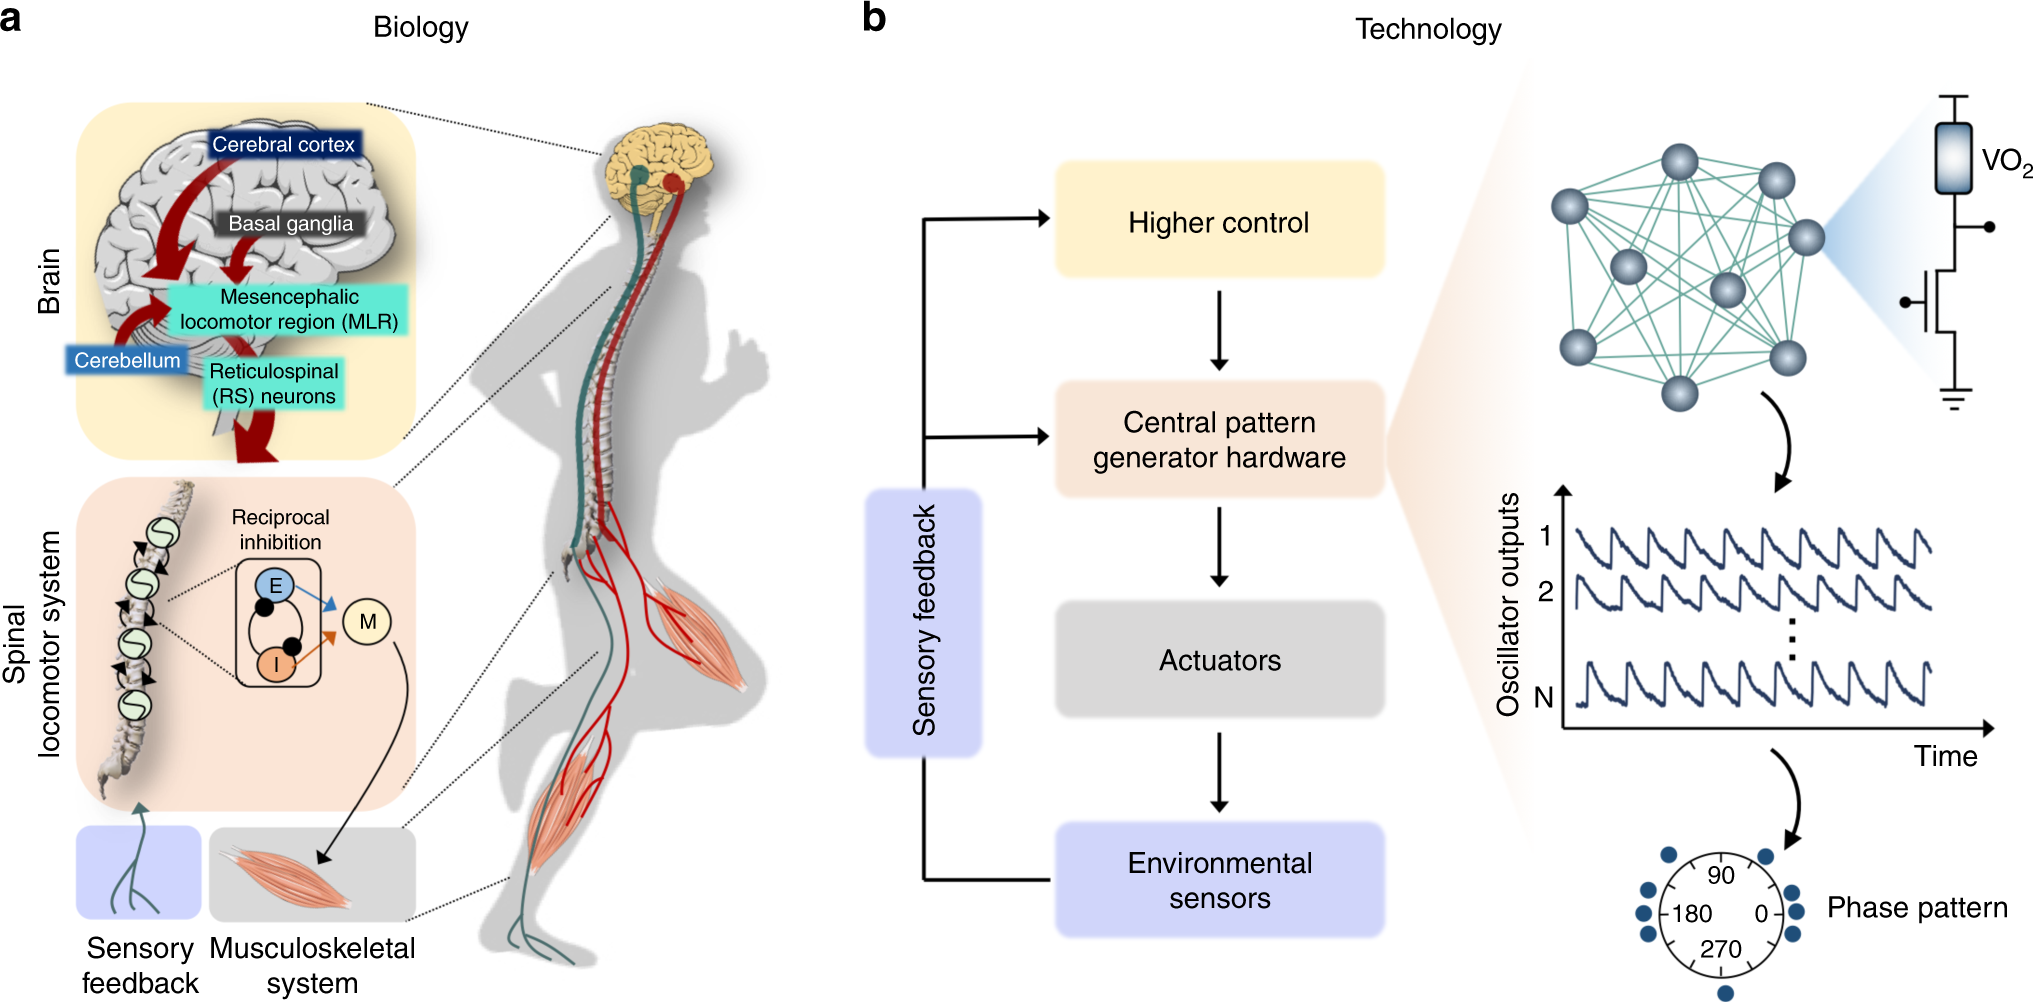
\includegraphics[width=\textwidth]{images/cpg_img.png}

\captionsource{Human locomotion system}{ https://www.nature.com/articles/s41467-019-11198-6/figures/1} \label{fig2}

\end{figure}

The movement of the animal, for example, cat, can be described as a sequence of phases stance and swing for limbs, where the stance is the duration of contact with the surface, and swing is the time in the air. As an animal moves faster, this cycle of phases shortens. Research by Halbertsma \cite{ref24_1} showed that it was mainly achieved by a decrease in stance duration while swing duration stayed mostly unchanged(example Fig.~\ref{fig3} ). Because phase-duration characteristics are integral property of motion initial test for synthetic CPG is to meet the same properties.

\begin{figure}
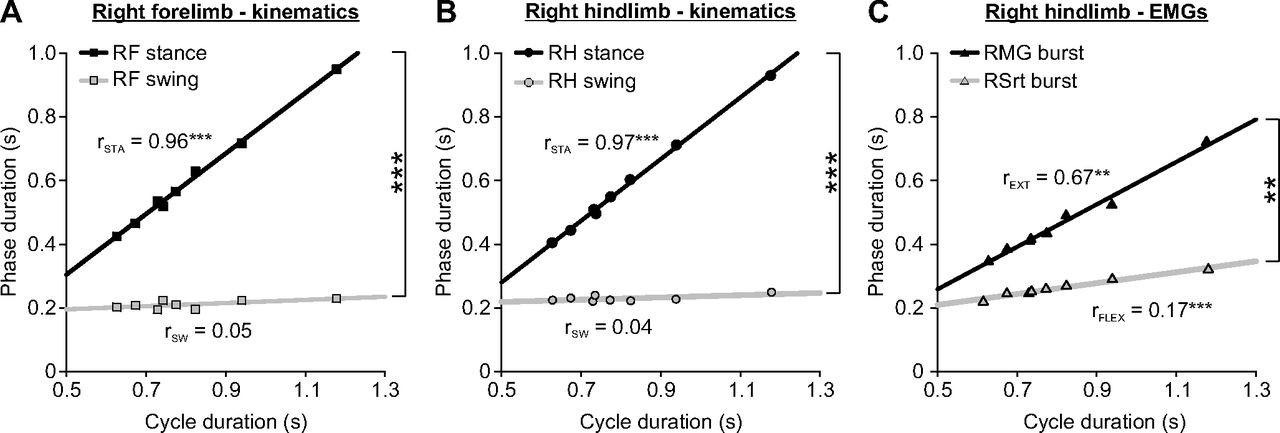
\includegraphics[width=\textwidth]{images/images_large_z9k0091424000003.jpeg}

\captionsource{Phase-duration characteristic}{ https://journals.physiology.org/cms/10.1152/jn.00524.2013/asset/images/large/z9k0091424000003.jpeg} \label{fig3}

\end{figure}


The task is to create a model that receives low dimensional input like the desired speed of an animal and produces a never-ending pattern in the same way that biological CPG does. We will use an average of 1000 steps from 9 different rats for the training and validation, which take up to 100 Gb of memory. The optimization task is to minimize the difference between real rat muscle neuron activation and generated one. Nengo framework will be used to build the CPGs model using SNNs. Spiking models are asynchronous, so input data has a time dimension. There are two ways data could be represented. In the first one, some random synchronized patterns with encoded speed will always feed to the network. Another approach would only give speed change signals once needed and empty signal any other time. There are also different approaches to train SNNs network. The research hypotheses is that SNNs could generalize well to biological CPGs.

\endinput 

\chapter{Data description}

In this chapter, we describe the nature of CPG data and its main characteristics. We are using these characteristics to generate synthetic data for training and validation. Below we provide a description of CPG data properties that helps to understand the main research questions.
 
\section{Locomotion phases}

Animal locomotion often described in terms of the gait cycle. A GC starts when a limb contacts the ground and ends when the same limb touches the ground next time. GC is usually broken into two stages: stance and swing. During a stance period, a limb is touching the ground as the opposite during swing phase limb is in the air. A swing phase distinguished from a stance phase when the last toes come off the ground. The intersection of swing phases for two limbs corresponds to running. 

\endinput
%\include{Chapters/Chapter4} 
%\include{Chapters/Chapter5} 

%----------------------------------------------------------------------------------------
%	THESIS CONTENT - APPENDICES
%----------------------------------------------------------------------------------------

\appendix % Cue to tell LaTeX that the following "chapters" are Appendices

% Include the appendices of the thesis as separate files from the Appendices folder
% Uncomment the lines as you write the Appendices

%
\chapter{Code}

\section{Pseudocode}

Something on the topic



\endinput
%\include{Appendices/AppendixB}
%\include{Appendices/AppendixC}
%----------------------------------------------------------------------------------------
%	BIBLIOGRAPHY
%----------------------------------------------------------------------------------------

\printbibliography[heading=bibintoc]

%----------------------------------------------------------------------------------------

\end{document}  
